%!TEX root =  ..\ekg_7_projektbericht.tex

%Realisierung/Akkumanagement und Versorgungsspannungen

\subsection{Akkumanagement und Versorgungsspannungen}

Dieses Unterkapitel behandelt die Umsetzung der Spannungsversorgung eines mobilen EKG Gerätes.

Bei der Auswahl eines Boost-Konvertes ist vor allem auf eine hohe Effizienz des ICs sowie einen geringen Eigenverbrauch zu achten. Darüber hinaus gibt es Boost-Konverter mit einem integrierten Enable Pin, welcher nicht nur den IC deaktiviert, sondern auch die Last vollständig vom Eingang abkoppelt. Dies ist überaus nützlich um im Standby Strom zu sparen. Ein Konverter der all diese Anforderungen erfüllt, ist der RP402N501F-TR-FE, welcher bereits ab 0,54€ im Falle einer Massefertigung erhältlich wäre, Ströme bis 800 mA sowie eine Effizienz von 90\% - 94\% unterstützt.
Die äußere Beschaltung dieses Wandlers beschränkt sich auf Pufferkondensatoren am Ein- und Ausgang, eine Induktivität zwischen dem Eingang und einem dedizierten Lx Pin und einem Pull-Down Widerstand am Enable Pin, welcher den IC auch im Fall einer deaktivieren MCU ausschaltet.

Betrachtet man den LDO ist zu beachten, dass ein dieser immer eine minimale Dropout Voltage hat, welche mindestens über ihn abfällt. Somit muss die Eingangsspannung größer als die gewünschte Ausgangsspannung plus Dropout Spannung sein. Würde man z.B. eine Ausgangsspannung von 3,3 V anstreben und der LDO eine Dropout Voltage von 0,2V besitzen, könnte man den Akku nur bis zu einer Spannung von 3,5 V entladen ohne die Ausgangsspannung zu beeinflussen. Dieser Umstand wird in Abbildung \ref{fig_DCDC_3V_plot} verdeutlicht. Deshalb wurde für das EKG-Gerät der LDO TPS79030DBVT mit einer niedrigen Dropout Spannung von 57 mV gewählt. Dieser LDO ist mit einer Restwelligkeit von 56 $\mu$V und einem Ruhestrom von 17 $\mu$A bestens zur Erfüllung der gestellten Ansprüche geeignet.

\begin{figure} [!h]
	%\centering
	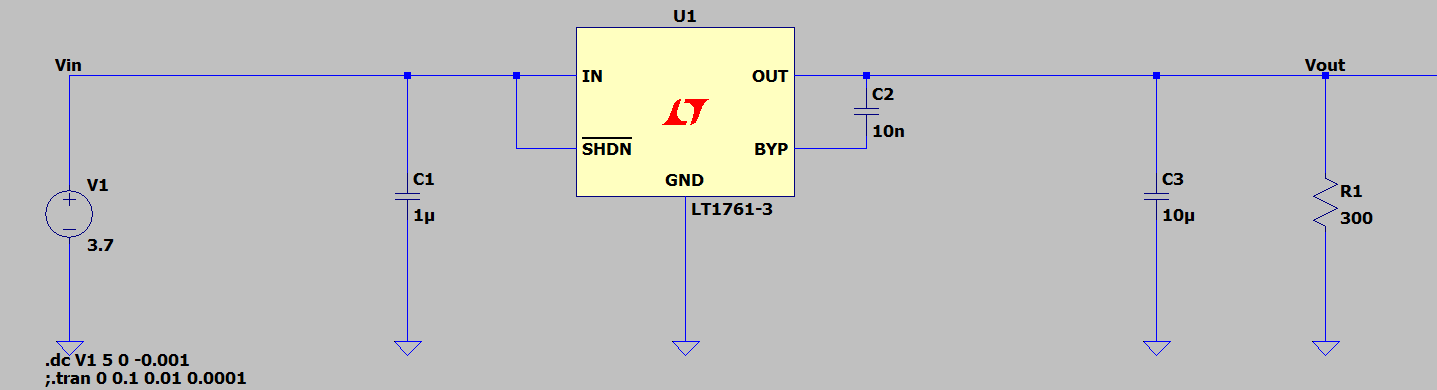
\includegraphics[width=\textwidth] {DCDC_3V_LDO_Shematic.png}
	\caption{Simulationsaufbau 3V LDO}
	\label{fig_DCDC_3V_sch} 
\end{figure}

\begin{figure} [!h]
	%\centering
	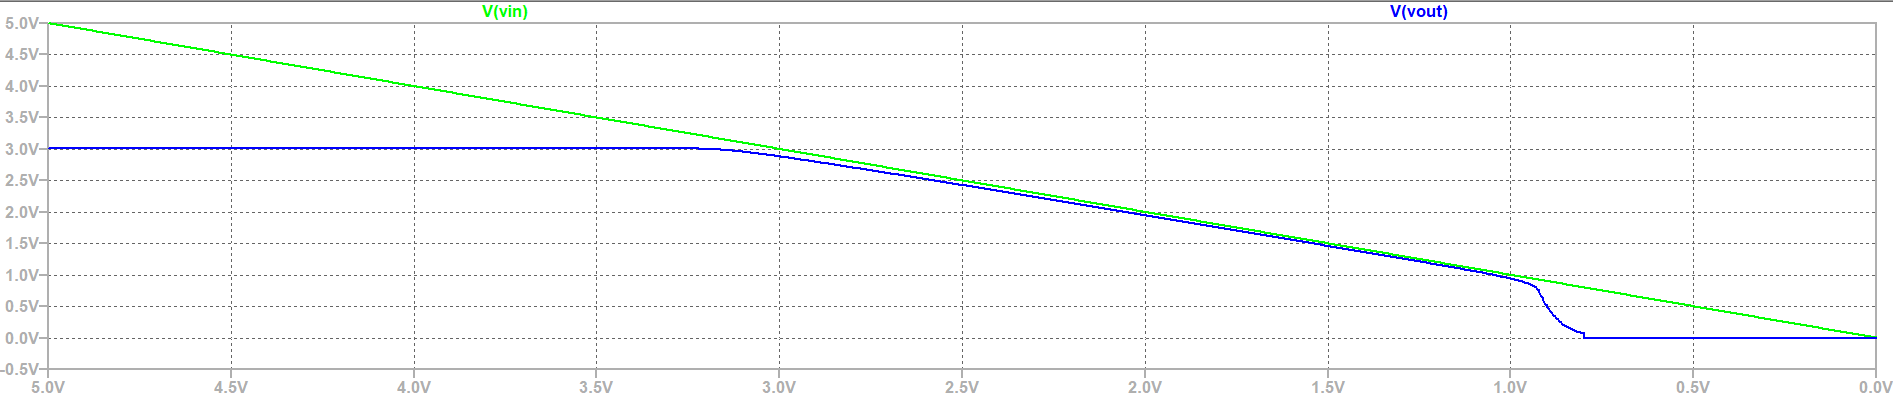
\includegraphics[width=\textwidth] {DCDC_3V_LDO_Plot.png}
	\caption{Ausgang 3V LDO mit fallender Eingangsspannung}
	\label{fig_DCDC_3V_plot} 
\end{figure}

Die Nutzung von Lithium-Ionen Zellen birgt einige Risiken. Mögliche Gefahren und getroffene Maßnahmen zur Reduktion dieser sind:

\begin{enumerate}
	\item Kurzschlüsse: \\
	Als erste Maßnahme hierfür ist der Anschluss der Batterie als Pin Header ausgeführt, wodurch sich am PCB seitigem Ende der Zuleitung eine Buchse befindet. Somit sind die Kontakte im inneren der Buchse geschützt und können nicht durch unachtsame Handhabung Kurzgeschlossen werden. Um bei Kurzschlüssen auf dem Board oder an der Peripherie den Akku zu schützen ist unmittelbar nach dem Header eine Sicherung platziert. Hierfür wurde aus der OMNI-BLOCK Serie von Littelfuse eine 1 Ampere Sicherung mit flinker Auslösecharakteristik gewählt (0154001.DRL). 
	
	\item Verpolung: \\
Um eine Beschädigung der Schaltung durch eine verkehrt eingesetzte Batterie zu verhindern, wodurch Plus- und Minuspol vertauscht wären, ist ein Verpolschutz durch einen PMOS vorhanden. Der Drain-Anschluss liegt hierbei an der Batterie währen der Source-Anschluss dem Rest der Schaltung zugewandt ist. Dadurch ist Bei korrekter Polung der Body-Diode von Drain nach Source leitend. Das Gate ist über einen Widerstand mit dem Ground verbunden, wodurch im Normalbetrieb eine negative Gate-Source Spannung anliegt und den Transistor komplett durchsteuert. Im Fall einer Verpolung ist die Body-Diode nicht leitend und es entsteht keine Potentialdifferenz zwischen Gate und Source. Der FET sperrt und die Schaltung ist geschützt.

	\item Überspannung:\\
	Überspannungen z.B. durch eine elektrostatische Entladung (ESD) beim wechseln der Batterie können der Schaltung Schaden zufügen. Zur Prävention ist am Spannungeingang eine Bidirektionale Transient Voltage Suppressor (TVS) Diode verbaut, welche Spannungen über 9V schnell nach Ground ableitet.
	
	\item Tiefenentladung:\\
	Eine Entladung auf Spannungen außerhalb der Spezifikation des Akkus können zu dessen Zerstörung führen. Aus diesem Grund wird fortwährend die aktuelle Akkuspannung des Geräts durch die MCU gemessen und ein Einschalten des Geräts wird nur bei ausreichender Spannung erlaubt. Zusätzlich wird ein Akku mit integrierter Schutzbeschaltung verwendet, welche ebenso einen Tiefentladungsschutz enthält.

\end{enumerate}

